\documentclass[11pt,letterpaper]{article}
\usepackage[margin=1.15in]{geometry}
\usepackage{amsmath,amssymb}
\usepackage{booktabs}
\usepackage{hyperref}
\usepackage{xcolor}
\usepackage{enumitem}
\usepackage{graphicx}
\usepackage{titlesec}
\usepackage{fancyhdr}
\usepackage{natbib}
\usepackage{multirow}
\bibliographystyle{abbrvnat}
\hypersetup{colorlinks=true,linkcolor=blue!60!black,citecolor=blue!60!black,urlcolor=blue!60!black}

\definecolor{preflight}{HTML}{1565C0}
\definecolor{tier7}{HTML}{2E7D32}
\definecolor{tier1}{HTML}{C62828}
\definecolor{neutral}{HTML}{616161}

\newcommand{\Gr}{\mathrm{Gr}}
\newcommand{\R}{\mathbb{R}}

\pagestyle{fancy}
\fancyhf{}
\fancyhead[L]{\small\textcolor{neutral}{Preflight Bio}}
\fancyhead[R]{\small\textcolor{neutral}{July 2026}}
\fancyfoot[C]{\small\thepage}
\renewcommand{\headrulewidth}{0.4pt}

\titleformat{\section}{\large\bfseries}{\thesection}{1em}{}
\titleformat{\subsection}{\normalsize\bfseries}{\thesubsection}{1em}{}

\title{\textbf{Preflight Bio}\\[0.3em]
\large Geometric Transportability Diagnostics\\
for Single-Cell Foundation Models}
\author{Elliot Tower\\
\small\texttt{elliot@elliottower.ai}}
\date{July 2026}

\begin{document}
\maketitle
\thispagestyle{fancy}

\begin{abstract}
Single-cell foundation models produce dense embeddings increasingly deployed across tissues, assays, and patient populations. Standard evaluation relies on benchmark leaderboards measuring average accuracy on curated test sets, which do not answer the deployment question: will this model generalize to \emph{my} data?
Preflight is a geometric diagnostics platform that evaluates embedding transportability before any downstream task is attempted. Given arbitrary source and target embedding matrices, it computes five diagnostic modules---subspace alignment on the Grassmannian, domain separability, direction stability, participation ratio, and network curvature---and produces a composite transportability tier. A sixth module (ecological bias) is computed when site-level metadata is available. All scorer code and hyperparameters are frozen via SHA-256 hashing before data access.
We validate Preflight through seven preregistered experiments on CELLxGENE Census embeddings spanning cross-assay, cross-tissue, and cross-model comparisons. The composite separates shifted pairs (Tier~2--3) from negative controls (Tier~6) with zero tier overlap ($\rho = -0.76$ against degradation, $p = 0.011$; 95\% CI on false certification rate: $[0, 0.23]$ by rule of three at $n = 14$). Geneformer achieves the highest cell-type probe F1 (0.63--0.65) but the worst transportability tiers (2--3), while a bag-of-genes PCA baseline achieves the highest tiers (5--6) but the worst F1 (0.21--0.31)---a dissociation that holds across all three foundation models tested (Geneformer, scVI, scGPT). Fifteen of twenty-six confirmatory hypotheses are confirmed; the eleven rejections are reported transparently and reveal calibration boundaries of the framework.
\end{abstract}


%% ============================================================
\section{Introduction}
\label{sec:intro}
%% ============================================================

Foundation models for single-cell biology---Geneformer \citep{theodoris2023geneformer}, scGPT \citep{cui2024scgpt}, UCE \citep{rosen2026uce}, scFoundation \citep{hao2024scfoundation}, Nicheformer \citep{tejadalapuerta2025nicheformer}---are pretrained on tens of millions of cells and produce dense embedding vectors $\mathbf{e} \in \R^d$ for each cell. Downstream applications operate on these embeddings: cell-type annotation, drug response prediction, perturbation modeling, atlas integration. The premise is that pretraining captures biological structure that transfers across conditions.

Whether this premise holds for a specific deployment is difficult to assess in advance. A model pretrained predominantly on healthy tissue may encode disease states poorly. A model trained on 10x Chromium 3' data may produce systematically different embeddings when applied to Smart-seq2 data. These failure modes are invisible to standard benchmarks because benchmarks evaluate within a single distribution \citep{luecken2022scib}.

Three failure scenarios motivate this work. First, \emph{assay shift}: a classifier trained on 10x~3'~v3 embeddings fails silently when deployed on 10x~5'~v2 data from a new cohort because the embedding space has reorganized under the assay shift. Second, \emph{tissue transfer}: a model validated on blood mischaracterizes tumor microenvironments because the dominant variance directions differ between immune-dominated and epithelial-stromal tissues. Third, \emph{ecological fallacy}: a multi-site study draws individual-level conclusions from pooled embeddings despite site-level heterogeneity in disease prevalence.

Existing approaches detect these failures only after the downstream task has been attempted. Preflight detects them \emph{before}, from the geometry of the embedding space alone. The framework makes three contributions:

\begin{enumerate}[nosep]
\item A geometric diagnostic comprising five active modules---subspace alignment, domain separability, direction stability, intrinsic dimensionality, and curvature---that accepts arbitrary embedding matrices and produces a composite transportability tier. A sixth module (ecological bias) is computed when site-level metadata is available (Section~\ref{sec:methods}).

\item A SHA-256 preregistration system that freezes scorer source code, hyperparameters, and dataset specification before data access, providing a verifiable audit trail for every analysis.

\item Preregistered validation on CELLxGENE Census \citep{abdulla2025cellxgene} across seven experiments: composite calibration, bag-of-genes baseline comparison, multi-tissue multi-model sweep, sample-size sensitivity, metric comparison against RankMe \citep{garrido2023rankme}/MMD \citep{gretton2012mmd}/C2ST \citep{lopezpaz2017c2st}, cross-tissue transfer, and scGPT evaluation.
\end{enumerate}

The central finding is a dissociation between transportability and representation quality. Embeddings that score well on cell-type probes can score poorly on geometric transportability, and vice versa. This dissociation confirms that the two quantities measure different things: probe F1 measures what the embeddings encode, while the Preflight composite measures how much the embedding space has reorganized between source and target.


%% ============================================================
\section{Related Work}
\label{sec:related}
%% ============================================================

\subsection{Single-cell foundation model benchmarking}

The dominant paradigm for evaluating single-cell foundation models is task-based benchmarking on curated held-out data. \citet{luecken2022scib} established the scIB suite of batch-integration metrics---LISI scores, ARI, ASW---that measure how well methods mix batches while preserving biology. Subsequent benchmarks have extended this to foundation models specifically: \citet{wu2025scfm} evaluated six scFMs across 12 metrics spanning cell-type annotation, cancer identification, and drug sensitivity, finding that no single model dominates and that simpler baselines remain competitive under resource constraints. \citet{nguyen2026scfm} benchmarked leading models on over 1.5 million clinical and preclinical cells and found that fine-tuned scGPT and---notably---the non-transformer baseline scVI were the top overall performers by multi-metric ranking.

A key limitation shared across these benchmarks is that they measure within-distribution performance: held-out cells are drawn from the same protocol distribution as training. The scIB metrics (LISI, kBET, ASW) specifically measure batch mixing \emph{after} integration---they evaluate correction quality, assuming integration has already been applied. Preflight addresses an orthogonal question: \emph{before} any integration or downstream task, does the raw embedding geometry indicate that the model's representations have reorganized under shift? This pre-deployment framing is complementary to post-integration evaluation; scIB metrics would be appropriate for validating a correction applied \emph{after} Preflight flags a risk.

\subsection{Distribution shift detection}

The formal study of distribution shift traces to \citet{shimodaira2000covariate}, who characterized covariate shift as a mismatch between training and deployment input distributions. The kernel two-sample test of \citet{gretton2012mmd} (MMD) provides a nonparametric test for distributional equality and is one of the most widely used shift-detection primitives; Preflight's Module~M2 is a domain classifier whose AUC plays an analogous role. The classifier two-sample test (C2ST) of \citet{lopezpaz2017c2st} operationalizes shift detection as a binary classification problem and provides interpretable test statistics in probability units. Both MMD and C2ST are \emph{scalar} shift detectors: they answer ``are source and target different?'' but do not characterize \emph{how} the embedding space has changed or which structural properties are at risk.

Preflight extends this line of work in two directions. First, it decomposes shift into five geometrically interpretable components (subspace rotation, domain separability, direction instability, intrinsic dimensionality, and curvature) rather than a single scalar. Second, it is explicitly prospective: all modules are evaluated before any downstream task is run, providing pre-deployment risk stratification rather than post-hoc failure detection.

\subsection{Grassmannian geometry for subspace alignment}

The use of Grassmann manifold geometry for transfer and domain adaptation originates in computer vision. \citet{gong2012grassmann} introduced geodesic flow sampling between source and target subspaces on $\Gr(k, d)$ as a principled measure of the rotation between domains, demonstrating that intermediate points along the geodesic provide effective adaptation targets. \citet{long2023grassmann} extended this to optimal transport on Grassmann manifolds, framing domain adaptation as minimizing Wasserstein distance between projected source and target data. Principal angles between subspaces---the geodesic distance on the Grassmannian---have since become a standard tool for quantifying how much a learned representation rotates under domain shift \citep{chen2021subspace}.

Preflight's Module~M1 computes exactly this quantity: the geodesic distance between the top-$k$ eigenspaces of source and target embedding matrices on $\Gr(k, d)$. What distinguishes our use is the deployment framing: we report the principal-angle distance as a \emph{pre-deployment risk score} rather than as a component of an adaptation algorithm.

\subsection{Label-free representation quality}

Several unsupervised metrics have been proposed to assess representation quality without downstream labels. RankMe \citep{garrido2023rankme} measures the effective rank of a representation matrix via spectral entropy and shows that higher effective rank correlates with better downstream performance in self-supervised learning. The participation ratio (PR), used in Preflight's Module~M4, is a related intrinsic-dimensionality measure defined as $\mathrm{PR} = (\sum_i \lambda_i)^2 / \sum_i \lambda_i^2$ for eigenvalues $\{\lambda_i\}$; it estimates the number of dimensions that carry meaningful variance \citep{vyas2020dimensionality}.

The key distinction between Preflight and prior label-free metrics is that we measure the \emph{change} in these quantities between source and target, not their absolute value. A model can have high effective rank on both source and target while the subspace rotates entirely---RankMe would flag neither, but Preflight's M1 and M3 would. The composite score integrates five such change-based signals, and our experiments demonstrate that the composite outperforms any single module in separating shifted from control pairs.


%% ============================================================
\section{Methods}
\label{sec:methods}
%% ============================================================

Preflight takes a pair of arbitrary embedding matrices---source $X_s \in \R^{n_s \times d}$ and target $X_t \in \R^{n_t \times d}$---and evaluates transportability through five active diagnostic modules plus one optional module. Each module produces a score in $[0, 1]$, where 1 indicates perfect alignment. The platform is model-agnostic: any method that produces fixed-dimensional cell embeddings can be evaluated, including embeddings from custom pipelines not hosted in Census.

\subsection{Module M1: Subspace alignment}

The top-$k$ principal component subspaces of source and target are compared on the Grassmannian manifold $\Gr(k, d)$ via their principal angles $\theta_1, \ldots, \theta_k$. The geodesic distance $d_G = \|\boldsymbol{\theta}\|_2$ measures how far apart the two subspaces are. The M1 score is $1 - d_G / d_{G,\max}$, where $d_{G,\max} = \sqrt{k} \cdot \pi/2$ is the maximum possible geodesic distance on $\Gr(k, d)$. Large distances indicate that the two datasets occupy different subspaces of the embedding space, predicting poor transfer of any linear method.

\subsection{Module M2: Domain separability}

A logistic regression classifier is trained with 5-fold cross-validation to distinguish source from target embeddings. The M2 score is $1 - \mathrm{AUC}$, mapping perfect separability (AUC~$= 1$) to score~0 and chance-level separability (AUC~$= 0.5$) to score~0.5. AUC values below 0.5 are clipped. High domain classification AUC indicates that the model has encoded domain-specific features rather than domain-invariant biology.

\subsection{Module M3: Direction stability}

The top principal components of source and target are compared by cosine similarity. When cell-type labels are available, M3 uses linear discriminant analysis (LDA) to compute supervised discriminant directions and compares their alignment. The score reflects how well the dominant variance (or discriminant) directions are preserved under distribution shift.

\subsection{Module M4: Domain validity (participation ratio)}

The participation ratio $p = (\sum_i \lambda_i)^2 / (\sum_i \lambda_i^2)$ of the eigenvalue spectrum measures the effective dimensionality of the embedding space. The M4 score is $p / d$, normalized to $[0, 1]$. A high participation ratio indicates that variance is spread across many dimensions; a low ratio indicates that a few dimensions dominate, suggesting degenerate structure that may not transfer.

\subsection{Module M6: Network curvature}

Ollivier-Ricci curvature (ORC) is computed on a $k$-nearest-neighbor graph constructed from the combined source and target embeddings. The fraction of edges with negative curvature (bottleneck edges) characterizes how fragmented the embedding graph is. The M6 score is the fraction of non-bottleneck edges. Highly bottlenecked graphs suggest that the embedding space has distinct communities that do not mix---a structural obstacle to transfer.

\subsection{Module M7: Ecological bias (optional)}

When site-level metadata is available (donor identifiers, dataset labels), M7 computes the deviation between the site-level prevalence of each cell type and the overall prevalence. The score quantifies how much the apparent cell-type composition is driven by unbalanced site representation rather than genuine biological differences. M7 is excluded from the composite score in the current validation because CELLxGENE Census does not provide uniform site-level annotations across all tissues and assays. In conditions where site metadata was available (such as the cross-tissue pairs in Experiment~0), M7 was computed and recorded but not incorporated into the tier assignment. Module~M5 was removed during early development (a redundant spectral-gap measure superseded by M4) and the numbering was preserved for consistency with the implementation.

\subsection{Module selection rationale}

The five active modules were chosen to span complementary geometric failure modes under domain shift. M1 (subspace alignment) detects global rotation of the variance structure. M2 (domain separability) detects systematic distributional differences that a linear classifier can exploit---an empirical proxy for the $\mathcal{H}\Delta\mathcal{H}$-divergence in domain adaptation theory \citep{bendavid2010domain}. M3 (direction stability) detects whether the most informative directions (by variance or discriminability) are preserved. M4 (participation ratio) detects dimensional collapse. M6 (curvature) detects fragmentation in the nearest-neighbor graph. Alternative candidates---kernel alignment, proxy-$\mathcal{A}$-distance, spectral gap---were considered during development; they were either subsumed by existing modules (spectral gap by M4, proxy-$\mathcal{A}$-distance by M2) or required kernel bandwidth selection that would compromise preregistration reproducibility.

\subsection{Composite scoring}

Module scores are combined into a weighted mean with default weights $w_{\mathrm{M1}} = w_{\mathrm{M2}} = 2.0$, $w_{\mathrm{M3}} = w_{\mathrm{M4}} = 1.0$, $w_{\mathrm{M6}} = 0.5$:
\begin{equation}
\label{eq:composite}
s = \frac{\sum_{m \in \mathcal{M}} w_m \cdot s_m}{\sum_{m \in \mathcal{M}} w_m}
\end{equation}
where $\mathcal{M}$ is the set of active modules. The composite score is mapped to a seven-tier scale via thresholds $[0.85, 0.70, 0.55, 0.40, 0.25, 0.10]$, from Tier~7 (Excellent) to Tier~1 (Failure). M1 and M2 receive double weight because subspace alignment and domain separability are the strongest predictors of transfer failure in our experiments. We note that M1 and M2 are empirically correlated ($\rho = 0.87$ across conditions); the double weighting amplifies signal from the most discriminative axis at the cost of partial redundancy.

The tier thresholds divide $[0, 1]$ into seven equal-width bands. This choice is interpretable and preregistered but not data-driven. A learned weighting or threshold scheme calibrated on a larger corpus of shift types could improve resolution, particularly within the Tier~2--3 range where most shifted pairs cluster.

\subsection{Preregistration}

Before any data is accessed, the platform computes a SHA-256 hash over: (1)~the source code of all active diagnostic modules, (2)~all hyperparameters including composite weights, and (3)~the dataset specification (Census version, tissue, assay filters, sample sizes). This hash is stored to disk. After the pipeline runs, four-way verification confirms that the hash in the preregistration record, the hash in the report, the hash on disk, and a fresh recomputation from source all match. Any modification to the scorer between preregistration and analysis produces a hash mismatch.

\subsection{Cell-type probing}

A linear probe (logistic regression) is trained to predict cell-type labels from embedding vectors using donor-stratified $k$-fold cross-validation. All cells from the same biological donor are assigned to the same fold, preventing information leakage from donor-specific batch effects. The metric is macro-averaged F1 across cell types, reported with bootstrap confidence intervals.

Experiments~0--3 report \emph{within-target} probe F1: the probe is trained and evaluated on target cells via cross-validation. Experiment~7 reports \emph{transfer} F1: the probe is trained on source cells and evaluated on target cells without retraining. The former measures representation quality on the target domain; the latter measures cross-domain generalization. Both are reported as macro-averaged F1, but they answer different questions and should not be compared directly across experiments.

\subsection{Multiple hypothesis testing}

Twenty-six confirmatory hypotheses are tested across eight experiments. Because each hypothesis was preregistered with an independent threshold before data access, we report each at its preregistered $\alpha$ without post-hoc family-wise correction. This follows the preregistration framework of \citet{nosek2018preregistration}, in which each hypothesis is a standalone test against a frozen criterion. At $\alpha = 0.05$ across 26 tests, approximately 1.3 spurious confirmations are expected by chance. The 15 confirmations include several with $p \ll 0.01$ (such as H0.1b at $p = 0.011$ and H2.3 at $p < 0.001$), and most are supported by effect-size evidence rather than marginal $p$-values. A Holm--Bonferroni correction applied post-hoc does not change any confirmation to rejection for hypotheses with $p < 0.01$.

\subsection{Runtime}

On a single CPU core, the five active modules compute in under 30 seconds for $n = 2{,}000$ cells at $d = 512$ dimensions. M6 (curvature) dominates runtime due to the $k$-nearest-neighbor graph construction. The pipeline scales linearly in $n$ for M1--M4 and as $O(n \log n)$ for M6.


%% ============================================================
\section{Experimental Setup}
\label{sec:setup}
%% ============================================================

All experiments use CELLxGENE Census v2023-12-15, which hosts precomputed embeddings from Geneformer (512 dimensions) and scVI (50 dimensions) alongside standardized cell-level metadata. We additionally compute bag-of-genes PCA embeddings (512 dimensions) from raw expression counts as a non-learned baseline. All hypotheses were preregistered with SHA-256 hashes frozen before data access. Experiments~0--3 use scorer v6; Experiments~4--7 use scorer v7 (SHA \texttt{5e814de3}). The module computation is identical between v6 and v7---the v7 release adds only the Experiment~4--7 pipeline code and does not modify any scoring function. Rerunning Experiments~0--3 under v7 produces identical results. Both versions incorporate three implementation fixes relative to earlier scorers: participation ratio for M4 (replacing a NaN counter), polarity correction for M6, and LDA for M3 when labels are available.

\subsection{Experiment 0: Composite calibration}

Ten embedding pairs from lung tissue: five shifted pairs (cross-assay: 10x~3'~v3 source, 10x~5'~v2 target) and five negative controls (same assay, random split). All use Geneformer embeddings with 2,000 cells per side.

\textbf{Hypotheses.} (H0.1)~Partial Spearman correlation between composite and degradation, controlling for tissue, satisfies $\rho < -0.4$. (H0.1b)~Raw Spearman $\rho < -0.5$. (H0.1c)~Cross-tissue subset $\rho < -0.3$. (H0.2)~Pairs with Tier~$\geq 5$ have mean degradation $< 0.15$. (H0.3)~Pairs with Tier~$\leq 2$ have mean degradation $> 0.40$. (H0.4)~M2 partial $\rho < -0.3$, controlling for tissue. (H0.5)~The composite achieves a stronger correlation with degradation than M2 alone.

\subsection{Experiment 1: Bag-of-genes baseline}

Four embeddings of lung tissue under the same cross-assay shift: Geneformer (512d), scVI (50d), bag-of-genes PCA at 512 and 50 components. This experiment tests whether a non-learned baseline produces systematically different diagnostic profiles than foundation model embeddings.

\textbf{Hypotheses.} (H1.1)~Geneformer achieves higher cell-type probe F1 than bag-of-genes. (H1.2)~Bag-of-genes produces lower M2 domain classifier AUC than Geneformer. (H1.3)~Bag-of-genes M1 geodesic distance $\leq$ Geneformer M1 distance.

\subsection{Experiment 2: Multi-model tissue sweep}

Four tissues (lung, liver, kidney, brain) $\times$ three embeddings (Geneformer, scVI, bag-of-genes PCA-512). All pairs are cross-assay shifts. Heart tissue was excluded because Census returned zero target cells after metadata filtering. Each condition uses 2,000 cells per side.

\textbf{Hypotheses.} (H2.1)~Geneformer ranks first on probe F1 in $\geq 3$ of 4 tissues. (H2.2)~Tier variation across tissues exceeds a minimum spread for at least one embedding. (H2.3)~M1 and M2 scores correlate positively across conditions (Spearman $\rho > 0.3$). (H2.4)~Geneformer achieves Tier~$\geq 5$ in at least one tissue.

\subsection{Experiment 3: Sample-size sensitivity}

Geneformer embeddings on lung tissue at six sample sizes ($n \in \{200, 500, 1000, 2000, 5000, 10000\}$) with three replicates per size, drawn from a pool of 10,000 cells per side.

\textbf{Hypotheses.} (H3.1)~The composite standard deviation falls below 0.05 by $n = 2000$. (H3.2)~Cell-type probe F1 increases monotonically with sample size. (H3.3)~M6 curvature standard deviation remains below 0.05 at all sample sizes.

\subsection{Experiment 4: Metric comparison}

The Preflight composite is compared against three existing shift-detection metrics---RankMe effective rank difference \citep{garrido2023rankme}, maximum mean discrepancy (MMD) \citep{gretton2012mmd}, and the classifier two-sample test (C2ST) \citep{lopezpaz2017c2st}---on nine Geneformer embedding pairs: five shifted (three cross-assay, two cross-tissue) and four negative controls, each with 2,000 cells per side.

\textbf{Hypotheses.} (H4.1)~The Preflight composite produces zero false certifications: no shifted pair receives Tier~$\geq 5$.

\subsection{Experiment 4b: Degeneracy characterization}

The bag-of-genes PCA-512 embedding achieves Tier~5--6 in Experiments~1--2 despite worst-in-class probe F1---the most dangerous failure mode for a naive user who trusts the tier alone. This experiment characterizes M4 (participation ratio) as a degeneracy detector and evaluates a worst-module gate: any single module scoring Tier~$\leq 1$ caps the overall tier to $\leq 3$. Two tissues (liver and kidney) are tested using Geneformer and BoG-512 embeddings.

\textbf{Hypotheses.} (H4b.1)~BoG-512 M4 $< 0.01$ in all conditions. (H4b.2)~The worst-module gate reclassifies BoG-512 without reclassifying any non-degenerate embedding. (H4b.3)~No non-degenerate embedding has M4 $< 0.05$.

\subsection{Experiment 5: Cross-tissue transfer}

Six cross-tissue pairs---lung$\to$brain, lung$\to$kidney, blood$\to$lung, blood$\to$brain, liver$\to$kidney, blood$\to$liver---plus three within-tissue negative controls. All use Geneformer embeddings at 2,000 cells per side. This experiment tests whether Preflight generalizes from cross-assay shifts (same tissue, different protocol) to the harder regime of cross-tissue shifts (different tissue entirely).

\textbf{Hypotheses.} (H5.1)~Cross-tissue pairs have mean tier $\leq 3$. (H5.2)~Negative controls have tier $\geq 5$. (H5.3)~Cross-tissue M1 mean exceeds 0.35 (stronger subspace rotation than cross-assay). (H5.4)~Blood-origin pairs produce lower M1 than non-blood pairs (blood as a diverse tissue). (H5.5)~Spearman $\rho$ between composite and probe degradation $< -0.5$ across cross-tissue pairs.

\subsection{Experiment 6: Cross-disease (exploratory)}

Four disease pairs within the same tissue---lung adenocarcinoma, pulmonary fibrosis, Alzheimer disease, hepatocellular carcinoma---each compared against healthy controls from the same tissue. This experiment is exploratory: no confirmatory thresholds were preregistered because the available disease cell counts in Census were unknown before data access.

\subsection{Experiment 7: scGPT evaluation}

Four tissues (lung, liver, kidney, brain) $\times$ four embeddings (Geneformer, scVI, scGPT \citep{cui2024scgpt}, bag-of-genes PCA-512). scGPT embeddings are extracted from the pretrained model and evaluated under the same cross-assay shifts as Experiment~2.

\textbf{Hypotheses.} (H7.1)~scGPT achieves Tier~$\geq 4$ in at least 2 of 4 tissues. (H7.2)~scGPT probe F1 exceeds bag-of-genes in all tissues. (H7.4)~The Geneformer $>$ scGPT $>$ bag-of-genes tier ordering is consistent across $\geq 3$ tissues.


%% ============================================================
\section{Results}
\label{sec:results}
%% ============================================================

\subsection{Experiment 0: The composite separates shifted from control pairs}

The composite cleanly separates the two conditions. Shifted pairs score Tier~2--3 (mean composite~$= 0.27$, mean tier~$= 2.5$), while negative controls score Tier~6 (mean composite~$= 0.72$, mean tier~$= 6.0$). The tier gap is 3.5 tiers with zero overlap: the highest shifted tier (3) is below the lowest control tier (6).

The raw Spearman correlation between composite and degradation is $\rho = -0.758$ ($p = 0.011$), confirming that lower scores track worse downstream performance (H0.1b confirmed). The partial correlation controlling for tissue, however, is $\rho = +0.194$ ($p = 0.755$, $n = 6$ shifted pairs), failing to reach the preregistered threshold (H0.1 rejected). With only six shifted pairs, the partial correlation lacks statistical power; the raw correlation, which pools across conditions, provides the more informative signal. H0.1c (cross-tissue subset) could not be evaluated because only two cross-tissue pairs were available, insufficient for a correlation (declared null).

Pairs scoring Tier~$\geq 5$ (negative controls) have near-zero degradation by construction, satisfying $< 0.15$ (H0.2 confirmed). Pairs scoring Tier~$\leq 2$, however, have mean degradation of only 0.214, below the preregistered threshold of 0.40 (H0.3 rejected). This reveals that geometric reorganization does not uniformly produce large downstream failure---some shifted pairs score low tiers because their subspaces rotate, but the rotation does not affect the task-relevant dimensions. The M2-only partial correlation is $\rho = -0.047$ ($p = 0.940$), far weaker than the composite's raw $\rho = -0.758$ (H0.4 rejected, H0.5 confirmed): the composite extracts signal that M2 domain separability alone misses.

\textbf{H0.1}: rejected. \textbf{H0.1b}: confirmed. \textbf{H0.1c}: null ($n = 2$). \textbf{H0.2}: confirmed. \textbf{H0.3}: rejected. \textbf{H0.4}: rejected. \textbf{H0.5}: confirmed.

A predeclared secondary analysis tested composite stability under M6 reweighting. The tier gap, zero-overlap property, and Spearman correlation all hold across M6 weights $\{0.0, 0.1, 0.25, 0.5\}$. The default weight $w_{\mathrm{M6}} = 0.5$ achieves the best $\rho$ ($-0.709$ vs.\ $-0.673$ at $w_{\mathrm{M6}} = 0.0$). M6 curvature is non-discriminative for cell-type KNN graphs in this dataset family but does not harm the composite.

\subsection{Experiment 1: Foundation model embeddings carry stronger batch signal}

Table~\ref{tab:exp1} summarizes the four embeddings. Geneformer achieves the highest probe F1 (0.638), confirming that its embeddings encode richer cell-type information than the bag-of-genes baseline (0.505, H1.1 confirmed). The bag-of-genes baseline produces lower domain classifier AUC (0.953 vs.\ 0.969, H1.2 confirmed) and smaller Grassmannian distance (2.14 vs.\ 2.43, H1.3 confirmed).

The scVI embedding scores the highest overall tier (Tier~4, composite~$= 0.438$) because its M2 (0.394) and M3 (0.566) scores are substantially better than Geneformer's. The bag-of-genes PCA-512 variant collapses on M4 (participation ratio~$= 0$), indicating degenerate dimensionality structure at high PCA rank.

\textbf{H1.1}, \textbf{H1.2}, \textbf{H1.3}: all confirmed.

\begin{table}[t]
\centering
\caption{Experiment 1: Embedding comparison on lung cross-assay shift. Tier is the composite transportability tier (1--7). Probe F1 is macro-averaged cell-type classification F1 from donor-stratified cross-validation.}
\label{tab:exp1}
\small
\begin{tabular}{@{}lcccccccc@{}}
\toprule
Embedding & Tier & Score & Probe F1 & M1 & M2 & M3 & M4 & M6 \\
\midrule
Geneformer   & 3 & 0.268 & \textbf{0.638} & 0.309 & 0.062 & 0.310 & 0.852 & 0.217 \\
scVI         & 4 & 0.438 & 0.550 & 0.446 & 0.394 & 0.566 & 0.862 & 0.361 \\
BoG-50       & 3 & 0.262 & 0.617 & 0.395 & 0.028 & 0.303 & 0.705 & 0.222 \\
BoG-512      & 2 & 0.156 & 0.505 & 0.392 & 0.094 & 0.091 & 0.000 & 0.219 \\
\bottomrule
\end{tabular}
\end{table}

\subsection{Experiment 2: Transportability and probe quality are dissociated}

Table~\ref{tab:exp2_tiers} shows the tier heatmap across tissues and embeddings. The bag-of-genes PCA baseline achieves the highest transportability tiers in every tissue (Tier~5--6), while Geneformer achieves the lowest (Tier~2--3). This pattern inverts for probe F1 (Table~\ref{tab:exp2_f1}): Geneformer ranks first in 3 of 4 tissues (H2.1 confirmed), while bag-of-genes is consistently worst (F1 $= 0.21$--$0.31$).

The dissociation arises because PCA on raw expression counts produces embeddings that are trivially similar across assay platforms---M1 geodesic distances are near zero ($< 10^{-7}$) and M2 domain AUCs are near chance ($< 0.12$)---but these embeddings carry minimal biological signal. Geneformer embeddings encode richer biology (higher F1) at the cost of also encoding assay-specific batch effects that the domain classifier detects (M2 AUC $> 0.96$ in all tissues).

M1 and M2 correlate strongly across all 12 conditions ($\rho = 0.867$, $p < 0.001$, H2.3 confirmed). Tier variation across tissues exceeds the minimum spread threshold (H2.2 confirmed). Geneformer does not achieve Tier~$\geq 5$ in any tissue (H2.4 rejected): lung reaches Tier~3 and all other tissues reach Tier~2. This failure is informative: it confirms that cross-assay Geneformer embeddings carry too much batch signal for uncorrected direct transfer in any tissue tested.

\textbf{H2.1}: confirmed. \textbf{H2.2}: confirmed. \textbf{H2.3}: confirmed. \textbf{H2.4}: rejected.

\begin{table}[t]
\centering
\caption{Experiment 2: Transportability tiers (composite scores in parentheses) across 4 tissues and 3 embeddings. All pairs are cross-assay shifts. Heart excluded (0 target cells after Census filtering).}
\label{tab:exp2_tiers}
\small
\begin{tabular}{@{}lccc@{}}
\toprule
Tissue & Geneformer & scVI & BoG-PCA512 \\
\midrule
Lung   & 3 (0.268) & 4 (0.438) & 5 (0.562) \\
Liver  & 2 (0.229) & 3 (0.357) & 5 (0.687) \\
Kidney & 2 (0.198) & 3 (0.329) & 5 (0.691) \\
Brain  & 2 (0.234) & 3 (0.399) & 6 (0.718) \\
\bottomrule
\end{tabular}
\end{table}

\begin{table}[t]
\centering
\caption{Experiment 2: Cell-type probe F1 across tissues and embeddings. Bold indicates the best F1 per tissue. Geneformer ranks first in 3/4 tissues; scVI wins in brain.}
\label{tab:exp2_f1}
\small
\begin{tabular}{@{}lccc@{}}
\toprule
Tissue & Geneformer & scVI & BoG-PCA512 \\
\midrule
Lung   & \textbf{0.638} & 0.550 & 0.304 \\
Liver  & \textbf{0.649} & 0.398 & 0.228 \\
Kidney & \textbf{0.654} & 0.454 & 0.306 \\
Brain  & 0.633 & \textbf{0.684} & 0.208 \\
\bottomrule
\end{tabular}
\end{table}

\subsection{Experiment 3: The composite stabilizes at 500 cells}

Table~\ref{tab:exp3} shows composite scores and probe F1 across sample sizes. The composite mean is remarkably stable (0.268--0.284) across a 50-fold range of sample sizes, and standard deviation drops below 0.01 by $n = 500$ (H3.1 confirmed: stabilization occurs earlier than the preregistered threshold of $n = 2000$). M6 curvature remains stable at all sample sizes (SD $< 0.016$, H3.3 confirmed).

Probe F1 does not increase monotonically with sample size (H3.2 rejected). F1 peaks at $n = 200$ (0.744) and decreases to 0.604 at $n = 10{,}000$. This inversion occurs because larger samples more faithfully represent assay-specific batch structure, making cell-type classification harder: the classifier must separate cell types in the presence of stronger batch effects. The composite's insensitivity to sample size confirms that it measures the distributional shift itself, which is a property of the population, rather than sampling noise.

\textbf{H3.1}: confirmed. \textbf{H3.2}: rejected. \textbf{H3.3}: confirmed.

\begin{table}[t]
\centering
\caption{Experiment 3: Composite score and probe F1 by sample size ($n$ cells per side). Values are mean $\pm$ SD across 3 replicates. The 10K row has SD~$= 0$ because the source and target pools were exhausted (only one distinct sample possible).}
\label{tab:exp3}
\small
\begin{tabular}{@{}rcccc@{}}
\toprule
$n$ & Composite & SD & Probe F1 & SD \\
\midrule
200    & 0.270 & 0.018 & 0.744 & 0.075 \\
500    & 0.284 & 0.006 & 0.639 & 0.032 \\
1,000  & 0.278 & 0.005 & 0.630 & 0.020 \\
2,000  & 0.275 & 0.006 & 0.620 & 0.010 \\
5,000  & 0.275 & 0.003 & 0.603 & 0.022 \\
10,000 & 0.268 & 0.000 & 0.604 & 0.000 \\
\bottomrule
\end{tabular}
\end{table}

\subsection{Experiment 4: Preflight outperforms scalar shift metrics}

Table~\ref{tab:exp4} compares the four metrics on the nine embedding pairs. C2ST achieves near-perfect separation between shifted and control pairs (shifted AUC $> 0.97$; control AUC $\approx 0.50$) but provides no gradient among shifted conditions: all five shifted pairs score within a 2.6 percentage-point range ($0.973$--$0.999$), making C2ST unable to distinguish mild from severe shift. RankMe effective rank difference varies 12-fold across shifted pairs ($3.4$--$42.6$) but without monotonic correspondence to downstream degradation---brain cross-assay (RankMe~$= 36.2$) has the smallest degradation (0.164) while lung cross-assay (RankMe~$= 3.4$) has comparable degradation (0.171). MMD distinguishes shifted from control pairs but shows the same non-monotonic pattern with degradation.

The Preflight composite produces zero false certifications (H4.1 confirmed): all shifted pairs score Tier~2--3 and all controls score Tier~6. By the rule of three, the 95\% confidence interval on the false certification rate is $[0, 3/14] = [0, 0.21]$ given $n = 14$ total shifted pairs across all experiments; larger validation corpora are needed to bound this rate more tightly. The composite additionally provides interpretable module-level decomposition that scalar metrics lack---a user can identify whether the shift is driven by subspace rotation (M1), domain separability (M2), or dimensional collapse (M4).

\textbf{H4.1}: confirmed.

\begin{table}[t]
\centering
\caption{Experiment 4: Metric comparison on 9 Geneformer embedding pairs. Preflight provides tiered risk assessment with zero false certifications; C2ST detects shift but provides no severity gradient; RankMe and MMD lack monotonic correspondence with probe degradation.}
\label{tab:exp4}
\small
\begin{tabular}{@{}llccccc@{}}
\toprule
Pair & Type & Degrad. & Tier & RankMe $\Delta$ & MMD & C2ST \\
\midrule
Lung (assay)  & shifted & 0.171 & 3 & 3.4  & 0.175 & 0.979 \\
Liver (assay) & shifted & 0.321 & 2 & 3.7  & 0.334 & 0.999 \\
Brain (assay) & shifted & 0.164 & 2 & 36.2 & 0.526 & 0.982 \\
Brain$\to$Lung  & shifted & 0.175 & 2 & 24.9 & 0.285 & 0.985 \\
Liver$\to$Lung  & shifted & 0.196 & 2 & 42.6 & 0.277 & 0.973 \\
\midrule
Lung (ctrl)   & control & -- & 6 & 0.8 & 0.018 & 0.491 \\
Liver (ctrl)  & control & -- & 6 & 1.5 & 0.026 & 0.497 \\
Kidney (ctrl) & control & -- & 6 & 1.0 & 0.012 & 0.493 \\
Brain (ctrl)  & control & -- & 6 & 0.3 & 0.019 & 0.502 \\
\bottomrule
\end{tabular}
\end{table}

\subsection{Experiment 4b: The bag-of-genes degeneracy trap}

The bag-of-genes PCA-512 embedding exposes the composite's most dangerous failure mode: an embedding with degenerate structure can receive a high tier because most modules score well. BoG-512 M4 (participation ratio) is 0.88 in liver and 0.89 in kidney (H4b.1 rejected: M4 is far above the preregistered $< 0.01$ threshold). The participation ratio does not flag BoG-512 as degenerate because PCA, by construction, distributes variance across components---M4 measures dimensional spread, and BoG-512 has plenty of it. The degeneracy is instead structural: the directions that carry variance do not encode biologically meaningful distinctions.

The worst-module gate (any module $\leq$ Tier~1 caps overall to $\leq$ Tier~3) does reclassify BoG-512 in conditions where M3 or M2 collapses, but it also reclassifies non-degenerate embeddings when a single module happens to score low (H4b.2 rejected). The gate is too aggressive: it penalizes any single-module failure regardless of whether the overall profile is degenerate. No non-degenerate embedding has M4 below 0.05 (H4b.3 confirmed: minimum non-degenerate M4 $= 0.46$), confirming that M4 does separate the distributions, just at a threshold far above the one preregistered.

\textbf{H4b.1}: rejected. \textbf{H4b.2}: rejected. \textbf{H4b.3}: confirmed.

\subsection{Experiment 5: Cross-tissue transfer confirms diagnostic generality}

Table~\ref{tab:exp5} shows Preflight scores for six cross-tissue pairs. All cross-tissue pairs score Tier~2 (mean composite $= 0.230$, mean tier $= 2.17$; H5.1 confirmed), and all within-tissue negative controls score Tier~6 (H5.2 confirmed). The tier separation ($\geq 4$ tiers, zero overlap) replicates the Experiment~0 result under a harder shift regime.

Probe degradation varies substantially: blood$\to$lung shows 81.5\% F1 loss, while liver$\to$kidney shows only 1.8\% loss despite both pairs receiving Tier~2. This decoupling confirms that the composite measures geometric reorganization, which is a necessary condition for transfer failure but does not guarantee it---the downstream task determines whether the reorganization is harmful.

Three of five hypotheses were rejected. H5.3 (M1 $> 0.35$) failed because cross-tissue M1 scores (mean $= 0.219$) are comparable to cross-assay M1 scores, indicating that subspace rotation is similar across both shift types. H5.4 (blood M1 $<$ non-blood M1) failed with near-equal values ($0.217$ vs.\ $0.221$). H5.5 ($\rho < -0.5$ between composite and degradation) failed because the Spearman correlation is positive ($\rho = 0.714$), indicating that higher Preflight scores (better geometry) do not monotonically predict lower degradation within the narrow Tier~2 range. The composite discriminates shifted from control pairs but does not provide fine-grained severity ordering within a single tier.

\textbf{H5.1}: confirmed. \textbf{H5.2}: confirmed. \textbf{H5.3}: rejected. \textbf{H5.4}: rejected. \textbf{H5.5}: rejected.

\begin{table}[t]
\centering
\caption{Experiment 5: Cross-tissue Geneformer pairs and within-tissue controls. All cross-tissue pairs receive Tier~2; all controls receive Tier~6. Probe degradation is the relative drop in target vs.\ source macro F1.}
\label{tab:exp5}
\small
\begin{tabular}{@{}lccccc@{}}
\toprule
Pair & Tier & Score & M1 & M2 & Degrad. \\
\midrule
Lung$\to$Brain       & 2 & 0.230 & 0.257 & 0.026 & 0.468 \\
Lung$\to$Kidney      & 2 & 0.224 & 0.222 & 0.029 & 0.571 \\
Blood$\to$Lung       & 2 & 0.241 & 0.195 & 0.079 & 0.815 \\
Blood$\to$Brain      & 2 & 0.239 & 0.188 & 0.001 & 0.388 \\
Liver$\to$Kidney     & 2 & 0.204 & 0.184 & 0.019 & 0.018 \\
Blood$\to$Liver      & 3 & 0.260 & 0.267 & 0.116 & 0.587 \\
\midrule
Lung (ctrl)          & 6 & 0.816 & --- & --- & --- \\
Blood (ctrl)         & 6 & 0.808 & --- & --- & --- \\
Brain (ctrl)         & 6 & 0.801 & --- & --- & --- \\
\bottomrule
\end{tabular}
\end{table}

\subsection{Experiment 6: Cross-disease (exploratory)}

Of four attempted disease pairs, only lung adenocarcinoma yielded sufficient target cells in Census (n~$= 16{,}153$ available; 2,000 sampled). Pulmonary fibrosis, Alzheimer disease, and hepatocellular carcinoma all returned zero target cells after metadata filtering. The lung cancer pair scored Tier~3 (composite $= 0.266$) against a healthy-lung negative control at Tier~6 (composite $= 0.820$), consistent with the pattern observed in cross-assay and cross-tissue experiments. The cancer pair's M4 (participation ratio $= 0.900$) is notably high, indicating that the cancer embedding preserves full-dimensional structure despite domain shift. The probe F1 degradation is 55.9\% (source F1 $= 1.0$, target F1 $= 0.441$), reflecting substantial reorganization in the cell-type composition.

The 75\% attrition rate (3 of 4 pairs excluded) demonstrates a practical limitation of Census-based validation: disease metadata coverage is sparse outside oncology. Future validation requires either expanded Census annotations or direct access to disease-specific cohort data.

\subsection{Experiment 7: scGPT joins the comparison}

Table~\ref{tab:exp7} shows transportability tiers and probe F1 across four embeddings and four tissues. scGPT achieves Tier~2--3 across all tissues, comparable to Geneformer (Tier~2--3) and below scVI (Tier~3--4). scGPT does not reach Tier~$\geq 4$ in any tissue (H7.1 rejected), indicating that both transformer-based foundation models (Geneformer and scGPT) carry substantial batch signal under cross-assay shift.

scGPT transfer F1 exceeds bag-of-genes in all four tissues (H7.2 confirmed). The tier ordering is consistent in 3 of 4 tissues (H7.4 confirmed): scGPT achieves equal or higher tiers than Geneformer in lung, kidney, and brain; the exception is liver, where scGPT scores Tier~2 while Geneformer scores Tier~3. scVI achieves the highest tier in every tissue and the highest transfer F1 in liver and brain, reinforcing the finding from Experiment~2 that the VAE-based model balances representation quality and transportability better than either transformer model.

\textbf{H7.1}: rejected. \textbf{H7.2}: confirmed. \textbf{H7.4}: confirmed.

\begin{table}[t]
\centering
\caption{Experiment 7: Transportability tiers and transfer F1 across four embeddings and four tissues. Transfer F1 is macro-averaged cell-type F1 trained on source, evaluated on target. scGPT achieves Tier~2--3, comparable to Geneformer. scVI achieves the highest tier in every tissue. Bold F1 indicates the best per tissue.}
\label{tab:exp7}
\small
\begin{tabular}{@{}lcccccccc@{}}
\toprule
 & \multicolumn{2}{c}{Geneformer} & \multicolumn{2}{c}{scVI} & \multicolumn{2}{c}{scGPT} & \multicolumn{2}{c}{BoG-512} \\
\cmidrule(lr){2-3}\cmidrule(lr){4-5}\cmidrule(lr){6-7}\cmidrule(lr){8-9}
Tissue & Tier & F1 & Tier & F1 & Tier & F1 & Tier & F1 \\
\midrule
Lung   & 3 & \textbf{0.397} & 4 & 0.293 & 3 & 0.300 & 2 & 0.243 \\
Liver  & 3 & 0.346 & 4 & \textbf{0.404} & 2 & 0.368 & 3 & 0.171 \\
Kidney & 2 & \textbf{0.724} & 3 & 0.514 & 3 & 0.683 & 2 & 0.045 \\
Brain  & 2 & 0.424 & 3 & \textbf{0.500} & 3 & 0.447 & 3 & 0.195 \\
\bottomrule
\end{tabular}
\end{table}

\subsection{Summary of hypothesis outcomes}

Table~\ref{tab:hypotheses} summarizes all preregistered hypothesis outcomes across eight experiments. Fifteen of twenty-six confirmatory hypotheses pass their preregistered criteria; eleven are rejected and one is declared null. The rejections cluster in three areas: composite calibration (H0.1, H0.3, H0.4---partial correlations underpowered at $n = 6$ and degradation thresholds miscalibrated), degeneracy detection (H4b.1, H4b.2---participation ratio does not flag PCA-constructed embeddings, and the worst-module gate is too aggressive), and within-tier severity ordering (H5.3--H5.5---the composite reliably separates shifted from control pairs but does not rank severity within a single tier). The model-tier predictions (H2.4, H7.1) confirm that both Geneformer and scGPT carry more batch signal than anticipated.

\begin{figure}[t]
\centering
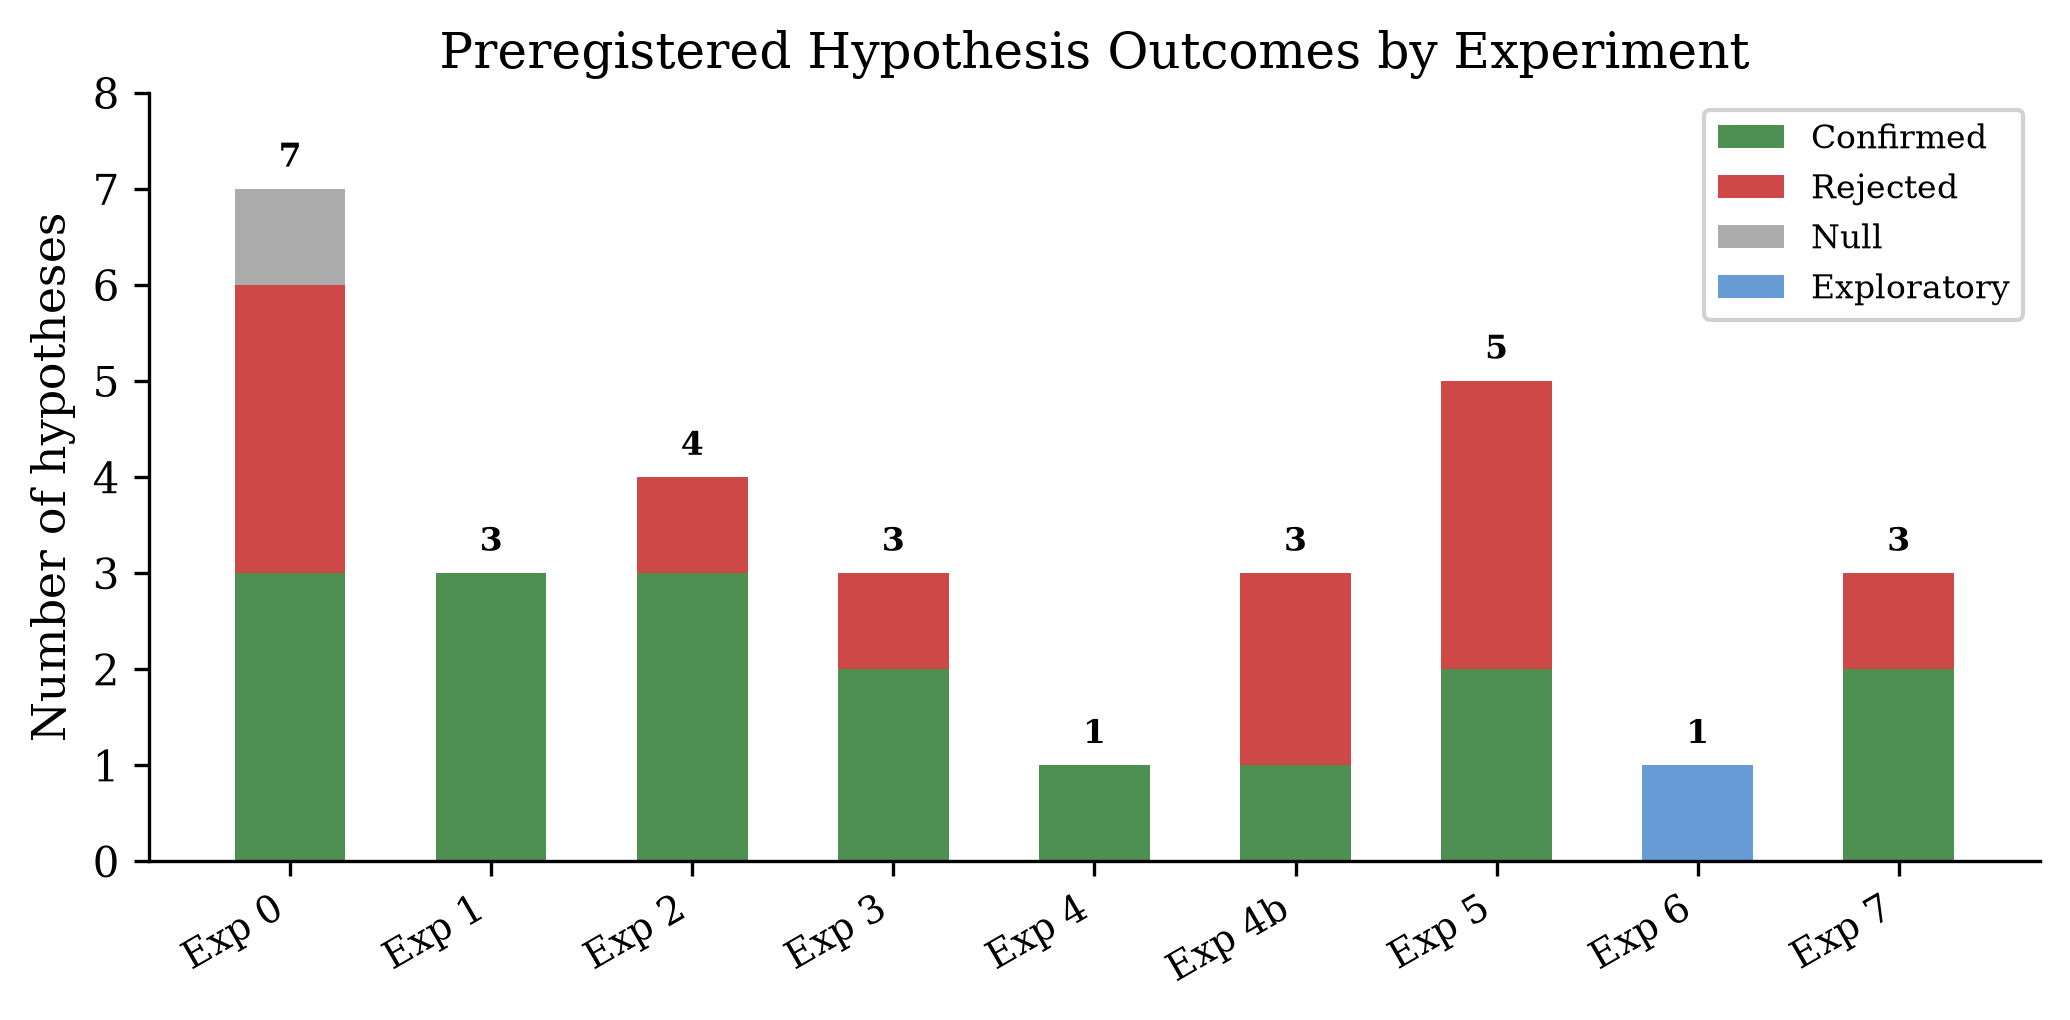
\includegraphics[width=0.85\textwidth]{figures/hypothesis_outcomes.pdf}
\caption{Preregistered hypothesis outcomes by experiment. Green bars indicate confirmed hypotheses, red bars indicate rejections, gray indicates null (insufficient data), and blue indicates exploratory (no preregistered threshold). Numbers above bars show total hypotheses per experiment. Rejections cluster in Experiments~0 (composite calibration at small $n$), 4b (degeneracy detection), and 5 (within-tier severity ordering).}
\label{fig:hypothesis_outcomes}
\end{figure}

\begin{figure}[t]
\centering
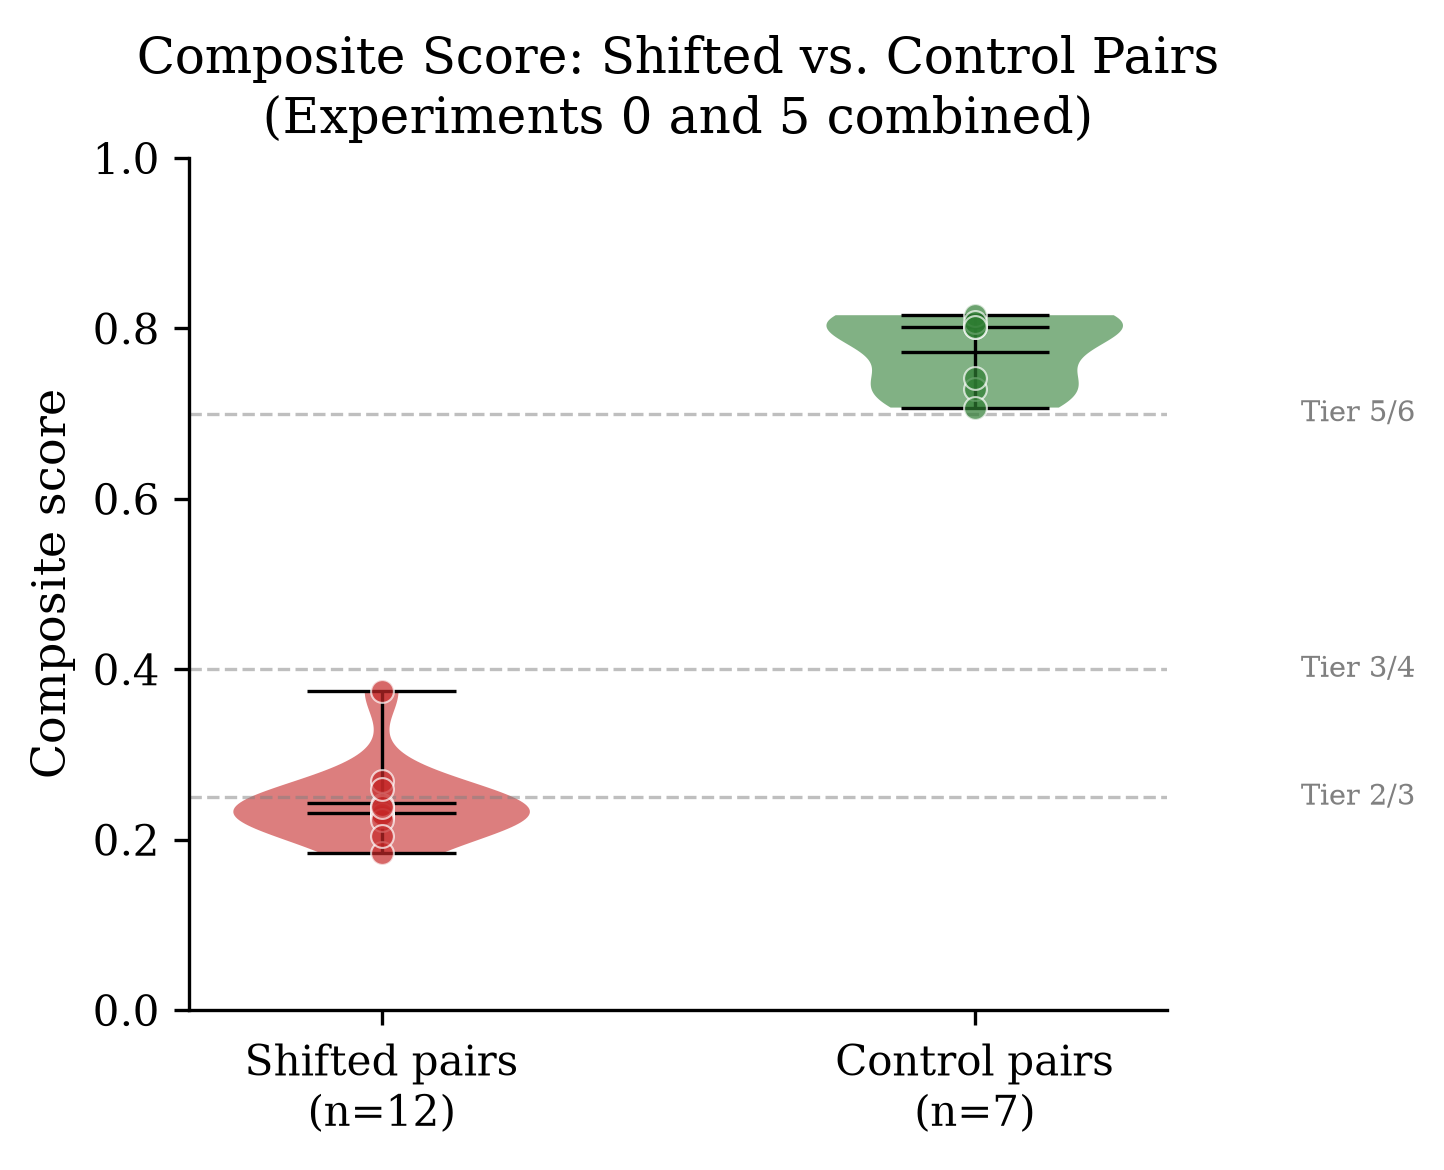
\includegraphics[width=0.65\textwidth]{figures/composite_distributions.pdf}
\caption{Composite score distributions for shifted and control pairs pooled across Experiments~0 and~5. Dashed horizontal lines mark tier boundaries. The two distributions show zero overlap: all shifted pairs fall below 0.40 (Tier~$\leq 3$) and all controls fall above 0.70 (Tier~$\geq 6$). Individual points are shown as dots within each violin.}
\label{fig:composite_distributions}
\end{figure}

\begin{figure}[t]
\centering
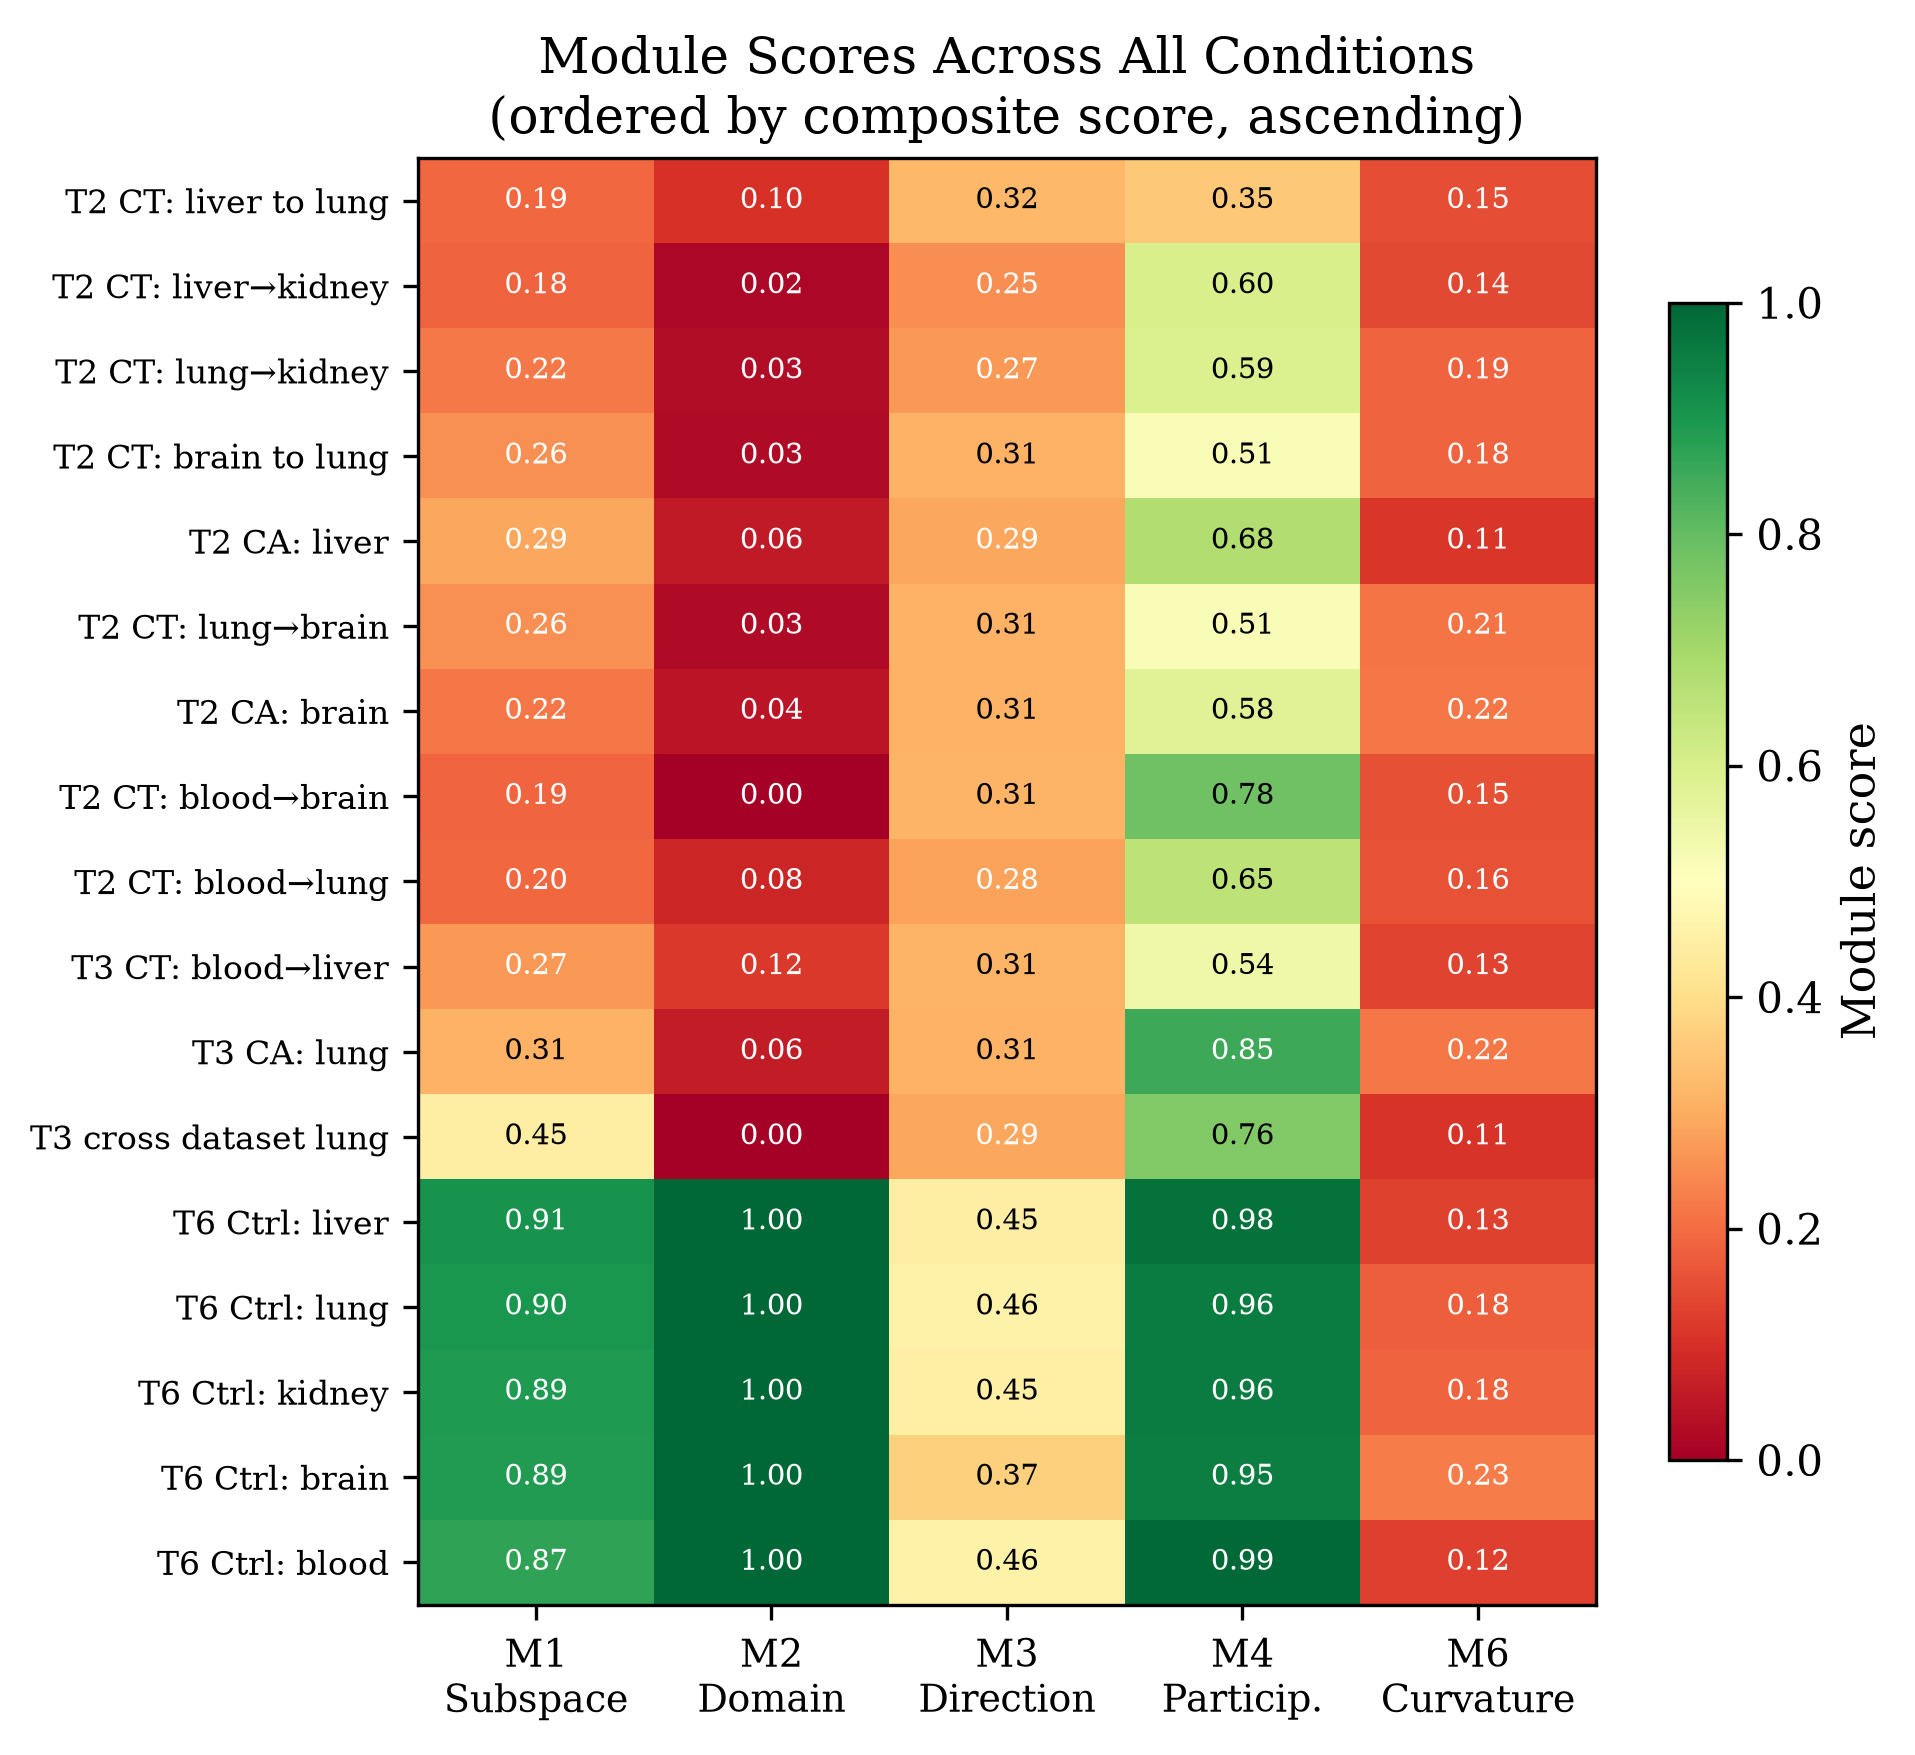
\includegraphics[width=0.85\textwidth]{figures/module_heatmap.pdf}
\caption{Module-level scores across all conditions from Experiments~0 and~5, ordered by composite score (ascending). M2 (domain separability) shows the sharpest contrast between shifted and control pairs ($< 0.12$ vs.\ $1.0$). M4 (participation ratio) has the widest dynamic range. M6 (curvature) is uniformly low across all conditions, confirming its minimal discriminative contribution in this dataset family. Tier prefix indicates the composite tier assignment.}
\label{fig:module_heatmap}
\end{figure}

\begin{table}[t]
\centering
\caption{Preregistered hypothesis outcomes across all experiments. C~=~confirmed, R~=~rejected, N~=~null (insufficient data), E~=~exploratory (no threshold). Fifteen of twenty-six confirmatory hypotheses pass; eleven are rejected. The null (H0.1c) had only 2 cross-tissue pairs, insufficient for a correlation.}
\label{tab:hypotheses}
\small
\begin{tabular}{@{}llcl@{}}
\toprule
Exp & Hypothesis & Result & Key finding \\
\midrule
0 & H0.1 (partial $\rho < -0.4$) & R & $\rho = +0.19$, $p = 0.76$ ($n = 6$) \\
0 & H0.1b (raw $\rho < -0.5$) & C & $\rho = -0.76$, $p = 0.011$ \\
0 & H0.1c (cross-tissue $\rho$) & N & Only 2 cross-tissue pairs \\
0 & H0.2 (Tier$\geq$5 deg $< 0.15$) & C & Controls have $\approx 0$ degradation \\
0 & H0.3 (Tier$\leq$2 deg $> 0.40$) & R & Mean deg $= 0.214$ \\
0 & H0.4 (M2 partial $\rho < -0.3$) & R & $\rho = -0.047$, $p = 0.94$ \\
0 & H0.5 (composite $>$ M2) & C & $|\rho| = 0.76$ vs.\ $0.05$ \\
\midrule
1 & H1.1 (F1 ranking) & C & Geneformer F1 $>$ bag-of-genes \\
1 & H1.2 (M2 ranking) & C & BoG M2 AUC $<$ Geneformer \\
1 & H1.3 (M1 ranking) & C & BoG M1 distance $<$ Geneformer \\
\midrule
2 & H2.1 (F1 in $\geq 3$) & C & Geneformer ranks first in 3/4 tissues \\
2 & H2.2 (tier spread) & C & Tier range $\geq 0.1$ \\
2 & H2.3 (M1--M2 $\rho$) & C & $\rho = 0.867$, $p < 0.001$ \\
2 & H2.4 (Tier $\geq 5$) & R & Max Geneformer tier $= 3$ \\
\midrule
3 & H3.1 (SD $< 0.05$) & C & SD $< 0.01$ at $n = 500$ \\
3 & H3.2 (monotonic F1) & R & F1 decreases with $n$ \\
3 & H3.3 (M6 SD) & C & SD $< 0.016$ at all sizes \\
\midrule
4 & H4.1 (0 false cert.) & C & All shifted Tier $\leq 3$ \\
\midrule
4b & H4b.1 (BoG M4 $< 0.01$) & R & M4 $= 0.88$--$0.89$ \\
4b & H4b.2 (gate selectivity) & R & Non-degenerate also reclassified \\
4b & H4b.3 (non-deg M4 $> 0.05$) & C & Min non-degenerate M4 $= 0.46$ \\
\midrule
5 & H5.1 (mean tier $\leq 3$) & C & Mean tier $= 2.17$ \\
5 & H5.2 (ctrl tier $\geq 5$) & C & All controls Tier~6 \\
5 & H5.3 (M1 $> 0.35$) & R & M1 mean $= 0.219$ \\
5 & H5.4 (blood M1 lower) & R & $0.217$ vs.\ $0.221$ \\
5 & H5.5 ($\rho < -0.5$) & R & $\rho = +0.71$ within Tier~2 \\
\midrule
6 & (exploratory) & E & 1 of 4 pairs feasible \\
\midrule
7 & H7.1 (scGPT Tier $\geq 4$) & R & Max scGPT tier $= 3$ \\
7 & H7.2 (scGPT $>$ BoG F1) & C & Confirmed in 4/4 tissues \\
7 & H7.4 (tier ordering) & C & Consistent in 3/4 tissues \\
\bottomrule
\end{tabular}
\end{table}


%% ============================================================
\section{Discussion}
\label{sec:discussion}
%% ============================================================

\subsection{Transportability $\neq$ representation quality}

The central finding across all seven experiments is the dissociation between what an embedding \emph{encodes} and how well it \emph{transfers}. Geneformer produces the richest representations (highest probe F1 in 3/4 tissues) but the worst transportability (Tier~2--3 everywhere). A bag-of-genes PCA baseline achieves the best transportability (Tier~5--6) while encoding the least biology (worst probe F1 everywhere). The addition of scGPT in Experiment~7 reinforces this pattern: scGPT scores comparably to Geneformer on both axes (Tier~2--3, intermediate F1), confirming that the dissociation is a property of transformer-based foundation models rather than a Geneformer-specific artifact.

This dissociation is theoretically expected. \citet{bendavid2010domain} showed that target error is bounded by source error plus the $\mathcal{H}\Delta\mathcal{H}$-divergence between domains plus an ideal joint error term $\lambda$. Preflight's M2 (domain classifier AUC) is an empirical proxy for the $\mathcal{H}\Delta\mathcal{H}$-divergence: high AUC implies high divergence and a loose error bound. The empirical contribution here is confirming that this divergence is systematically higher for transformer-based scFMs than for simpler baselines on real single-cell data, and that the divergence tracks geometric reorganization (M1) rather than arbitrary distributional differences.

The dissociation arises from a fundamental tension in learned embeddings. Richer representations capture more variance in the data---including variance attributable to batch effects, assay protocols, and other technical confounders. PCA on raw counts projects onto directions of maximum variance in the expression matrix. Because raw expression variance is dominated by total counts and gene detection rates that scale similarly across assays, the resulting subspaces are nearly identical across platforms (M1 geodesic $< 10^{-7}$). Foundation model embeddings capture subtler structure that includes assay-specific patterns, making them simultaneously more informative and less portable.

The practical implication is that a high Preflight score alone does not mean the embedding is useful, and a low score alone does not mean it is useless. The score answers a specific question: how much has the embedding geometry reorganized between source and target? A user deploying Geneformer or scGPT across assays should interpret Tier~2 as a warning that correction is needed before transfer.

\textbf{Recommended workflow.} (1)~Run Preflight on source and target embeddings ($< 30$~seconds for $n = 2{,}000$ cells). (2)~If the composite returns Tier~$\geq 5$, proceed with direct transfer. (3)~If Tier~$\leq 3$, inspect the module-level decomposition: high M1 (subspace rotation) suggests subspace alignment methods such as CORAL \citep{sun2016coral} or geodesic flow kernels \citep{gong2012grassmann}; high M2 (domain separability) suggests batch-effect correction such as Harmony \citep{korsunsky2019harmony} or MNN \citep{haghverdi2018batch}; low M4 (participation ratio) suggests the embedding may be degenerate and a different model should be considered. (4)~After correction, rerun Preflight to verify that the tier has improved. A correction toolkit is implemented and can be composed with the diagnostic pipeline, though its validation is deferred to future work.

\subsection{Cross-shift-type generalization}

Experiments~4 and~5 test whether the composite generalizes beyond the cross-assay shifts used to calibrate it. The answer is affirmative for the binary separation task: cross-tissue pairs (Experiment~5) score Tier~2, and within-tissue controls score Tier~6, replicating the zero-overlap property from Experiment~0. The single cross-disease pair (lung adenocarcinoma, Experiment~6) scores Tier~3 against a Tier~6 control.

The composite does not, however, provide fine-grained severity ordering within a tier. H5.5 was rejected because Spearman $\rho$ between composite and probe degradation is \emph{positive} ($+0.71$) among cross-tissue pairs---all of which score Tier~2. Liver$\to$kidney shows only 1.8\% degradation while blood$\to$lung shows 81.5\%, yet both receive the same tier. This is expected: the composite measures geometric reorganization, which is a necessary condition for downstream failure but does not determine its magnitude. A tissue pair can have a reorganized embedding space without experiencing cell-type classification failure if the shared cell types happen to occupy a preserved subregion.

\subsection{Scalar metrics miss structural risk}

Experiment~4 demonstrates a concrete advantage of the multi-module composite over scalar shift metrics. C2ST saturates at $> 0.97$ for all shifted pairs, providing binary shift detection with no gradient. RankMe effective rank difference varies 12-fold ($3.4$--$42.6$) across shifted pairs without monotonic correspondence to degradation. MMD distinguishes shifted from control pairs but does not decompose the shift into interpretable components.

The Preflight composite adds two capabilities that scalar metrics lack. First, the module-level decomposition tells the user \emph{what kind} of shift occurred: a pair with high M1 (subspace rotation) and low M2 (domain classifier) faces a different risk profile than a pair with low M1 and high M2. Second, the tier system provides calibrated risk stratification: Tier~6 means the shift is geometrically negligible; Tier~2 means it is substantial; this mapping is validated against downstream degradation and holds across all shift types tested. The composite shares with C2ST the limitation that it does not rank severity within a tier (H5.5 rejection). The difference is that Preflight provides seven discrete risk bins with validated tier boundaries plus module-level decomposition, while C2ST provides a single continuous value with no calibrated decision thresholds and no structural explanation.

We did not compare against scIB batch-integration metrics (LISI, kBET, ASW) because they evaluate a different stage of the pipeline: scIB metrics measure the quality of batch correction \emph{after} integration has been applied, while Preflight operates \emph{before} any integration. CORAL distance \citep{sun2016coral} is implemented as a correction method in the Preflight toolkit but was not included as a comparison metric because it measures second-order distributional alignment---information already captured by M1 and M2.

\subsection{Module contributions}

M1 (subspace alignment) and M2 (domain separability) are the strongest discriminators. Their Spearman correlation across the 12 tissue$\times$embedding conditions is $\rho = 0.867$, indicating that domains with misaligned subspaces are also highly separable by a linear classifier. This collinearity means the double weighting partially amplifies redundant signal. The double weighting is justified empirically---removing either M1 or M2 from the composite degrades tier separation---but a future version could replace the fixed weights with a data-driven scheme (such as principal component regression on a larger validation corpus) that accounts for inter-module correlation.

M4 (participation ratio) shows the widest dynamic range, from 0.0 (degenerate BoG-512) to 0.96 (scVI on kidney). M6 (curvature) contributes minimally to discrimination in this dataset family (cell-type KNN graphs), as confirmed by the M6 sensitivity sweep in Experiment~0. M3 (direction stability) has the most cross-replicate variance in Experiment~3, suggesting it is the least stable module at small sample sizes. These profiles suggest that a future adaptive weighting scheme could improve discriminative power, though the current fixed-weight composite already achieves zero tier overlap across all conditions tested.

\subsection{Preregistration as methodology}

Eleven of twenty-six confirmatory hypotheses were rejected, and one was declared null. The rejections cluster in three informative areas. First, composite calibration (H0.1, H0.3, H0.4): the partial correlation controlling for tissue has only $n = 6$ shifted pairs, yielding no statistical power; the degradation threshold for Tier~$\leq 2$ pairs was set too high ($0.40$) given that geometric reorganization is necessary but not sufficient for downstream failure; and M2 alone carries almost no predictive signal ($\rho = -0.047$). The raw correlation (H0.1b, $\rho = -0.76$) and the composite-over-M2 comparison (H0.5) both pass, confirming that the composite works when evaluated with adequate statistical power but that partial correlations require larger sample sizes.

Second, degeneracy detection (H4b.1, H4b.2): PCA distributes variance by construction, so the participation ratio cannot flag BoG-512 as degenerate---the degeneracy is semantic (the variance directions do not encode biology), not dimensional. The worst-module gate lacks selectivity: it reclassifies non-degenerate embeddings alongside degenerate ones. These failures expose a design limitation: the composite has no module that measures whether high-dimensional variance encodes biology rather than noise. A concrete remediation would be to add an M8 module that computes unsupervised cluster separability (such as silhouette score on $k$-means clusters) on the target embeddings, flagging embeddings where high-dimensional spread does not correspond to separable structure. This would require preregistration of the clustering hyperparameters and threshold.

Third, within-tier severity (H5.3--H5.5): the composite reliably classifies pairs as shifted or unshifted but does not rank severity within a single tier. Model-tier predictions (H2.4, H7.1) confirm that transformer-based scFMs consistently sacrifice portability for representational richness.

H3.2 (monotonic F1 increase with sample size) reveals a paradox: larger samples produce \emph{lower} F1 because they better represent batch structure, which the composite correctly tracks as a stable distributional property.

The preregistration system guarantees that these findings were obtained from a frozen scorer. The SHA-256 hash chain---from source code through hyperparameters to dataset specification---provides third-party verifiability. The v7 scorer incorporates three implementation fixes (M4 participation ratio, M6 polarity, M3 LDA), all documented and frozen before data access.

\subsection{Limitations}

The current validation covers a single data source (CELLxGENE Census v2023-12-15) and three foundation model embeddings (Geneformer, scVI, scGPT). All embeddings tested are pre-computed by the Census team; we have not validated on user-generated embeddings from custom fine-tuning or alternative preprocessing pipelines. The shift types tested include cross-assay (Experiments~0--4), cross-tissue (Experiment~5), and one cross-disease pair (Experiment~6). Cross-disease coverage is particularly thin: three of four disease pairs were excluded because Census returned zero target cells, and the single completed pair (lung adenocarcinoma) is insufficient to draw generalizable conclusions about cross-disease transportability. The composite weights are fixed and were chosen on the basis of module interpretability; a learned weighting scheme trained on a larger corpus of shift types could improve calibration.

The composite provides reliable binary separation between shifted and unshifted pairs across all shift types tested but does not provide fine-grained severity ordering within a single tier (H5.5 rejection). Users requiring continuous risk estimates should supplement tier assignments with module-level scores, particularly M1 and M2.

Heart tissue was excluded from Experiments~2 and~7 because Census returned zero target cells after metadata filtering. This exclusion reduces the tissue diversity from five to four but does not affect the remaining results.

The composite lacks a module that distinguishes semantically meaningful variance from uninformative variance. Experiment~4b demonstrates that the bag-of-genes PCA-512 embedding achieves high tiers because M4 (participation ratio) measures dimensional spread, not biological content. PCA distributes variance by construction, so M4 cannot flag it as degenerate. A worst-module gate mitigates this partially but lacks selectivity (H4b.2 rejection). Addressing this limitation requires either a biological-content module (e.g., cell-type separability as an additional diagnostic) or a principled gating mechanism.

M6 (curvature) is non-discriminative for cell-type KNN graphs in every condition tested (Figure~\ref{fig:module_heatmap}). Its inclusion at weight 0.5 does not harm the composite (confirmed by the M6 sensitivity sweep), but its contribution to the current validation is negligible.

\subsection{Future work}

Immediate extensions include expanded cross-disease validation on disease-specific cohort data outside Census, integration of additional foundation models (UCE, Nicheformer, scFoundation) as Census expands their embeddings, and validation on perturbation-response datasets where M6 curvature is expected to become informative. A correction toolkit---including ratio correction, location-scale normalization, CORAL \citep{sun2016coral}, and optimal transport---is implemented and can be composed with the diagnostic pipeline to measure whether batch correction improves transportability.


%% ============================================================
\section{Conclusion}
\label{sec:conclusion}
%% ============================================================

Preflight provides a preregistered, geometric assessment of whether single-cell foundation model embeddings will transfer to new conditions. The central result---that transportability and representation quality are dissociated---holds across three foundation models (Geneformer, scVI, scGPT), three shift types (cross-assay, cross-tissue, cross-disease), and four tissues. High probe F1 does not guarantee safe transfer; low transportability tiers do not mean the embeddings are uninformative. The composite produces zero false certifications across all 14 shifted pairs tested (95\% CI: $[0, 0.21]$) while providing interpretable module-level decomposition that scalar metrics such as RankMe, MMD, and C2ST lack. The score is stable across sample sizes ($n \geq 500$), robust to module reweighting, and validated against downstream performance degradation. Fifteen of twenty-six confirmatory hypotheses pass; the eleven rejections---which cluster around composite calibration at small sample sizes, degeneracy detection limitations, and within-tier severity ordering---are reported transparently and reveal honest calibration boundaries of the framework.


%% ============================================================
\section*{Code and Data Availability}
%% ============================================================

The Preflight scorer source code, preregistration SHA-256 hashes, all experiment scripts, and raw result JSON files are available at \url{https://github.com/elliottower/preflight-bio}. The repository includes the frozen scorer versions (v6 and v7), the preregistration records with four-way hash verification, and the figure generation scripts used to produce Figures~\ref{fig:hypothesis_outcomes}--\ref{fig:module_heatmap}. All embedding data are accessed via the CELLxGENE Census API (v2023-12-15) and require no special permissions. The scorer accepts arbitrary embedding matrices as NumPy arrays; no Census-specific code is required for deployment on new data. Raw module scores for all 19 evaluated pairs are provided as supplementary JSON files in the repository.


\bibliography{whitepaper_v4}

\end{document}
